  \section{Experiments}
\label{sec:experiments}

In this section, we describe our HBM implementation and Ramulator~\cite{Ramulator} simulations on several PARSEC~\cite{bienia09parsec2} benchmarks. We run the PARSEC v2.1 and v3.0 benchmarks suites with the gem5~\cite{parsec_2_1_m5} simulator to generate memory traces of multi-core shared-memory scenarios. Next, we evaluate the performance of the reorder buffer by running the memory traces through the Ramulator DRAM simulator. To evaluate the performance of our proposed memory system, we compare the number of CPU cycles needed to run the PARSEC memory traces through the original Ramulator program and an extended version of Ramulator which includes the memory system.

\subsection{HBM Implementation}
%\Ethan{Move all implementation details here, is sub-channel the same as pseudo channel? OK or still repetitive?}
%\Ankit{Suddenly, there is too much jargon about HBM...Have we defined all these things in the background section?}
Our coding scheme is based on a single $16$-bank channel of HBM DRAM operating in Pseudo Channel Mode ($8$ banks per pseudo channel). To fit the layout of Figure~\ref{fig:memsys} and Section~\ref{sec:codingArchitecture}, Pseudo Channel 0 is used for data banks and Pseudo Channel 1 is used for parity banks. 
%
%The pseudo channel conceptually divides the memory of a single channel in half. 
%Since this mode divides a channel into two individual $8$ bank sub-channels, we assign one sub-channel for data banks and the other sub-channel for parity banks. 
%
Wherever possible, we try to interleave the banks. This ensures that most large, linear accesses will be spread across multiple banks with reduced contention.

In this mode, the 128-bit data bus is split into 2 individual 64-bit segments. 
However, the pseudo channels share the same address and command bus: commands and addresses may be sent to one pseudo channel or the other, but not to both. They also decode and execute commands individually. For commands that are common to both pseudo channels, strict timing conditions must be met to avoid conflicts.
%The burst length is set to $4$. This means that on each segment, a read or write transaction transfers $256$ bits in a burst of four $64$-bit cycles. 
Table~\ref{tab:design_params} describes additional design details.
%
\begin{table}[h!]
 \small
  \centering
  \begin{tabular}{|c|p{5cm}|}
    \hline
    Memory overhead & Storage of parity is limited to 50\% of the overall memory. \\
    \hline
    Memory Banks & 8 Data banks, 8 parity banks \\
    \hline           
    Cache Line Size & 128/256 bytes size \\ \hline  
    Element Size & Each element is 256 bytes \\ \hline  
    Number of Cores & 6-8 cores for Wireless SoC platform \\ \hline  
    Access Rate & 1GHz memory speed \\ \hline  
    Burst Length & 4 (256-bit transfer in four 64-bit bursts)\\ \hline
  \end{tabular}
  \caption{Summary table of design parameters.}
  \label{tab:design_params}
\end{table}


\begin{remark} %[{\bf Address mapping}]
\label{rem:address}
%\Ankit{I don't see any reason to present address mapping here...or probably this needs to presented in a better manner to create coherent story.} 
Figure~\ref{fig:mapping} describes the address mapping for each channel. The least significant ``OFFSET'' bits of the address signify the byte level addressing of the data. The $6$ most significant ``CA'' bits indicate column address, the next $14$ ``RA'' bits indicate row address, the $3$ ``BA'' bits decide the bank, and the remaining $3$ ``CH'' bits specify the channel. 
\end{remark}
%%%%%%%%%%%%%%%%%%%%%%%%%%%%%%%%%%%%%%%%%%%
\begin{figure}[h!] \centering
%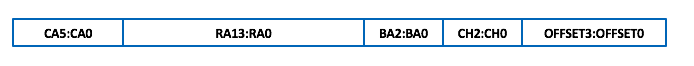
\includegraphics[width=0.95\linewidth]{figures/mapping.png} 
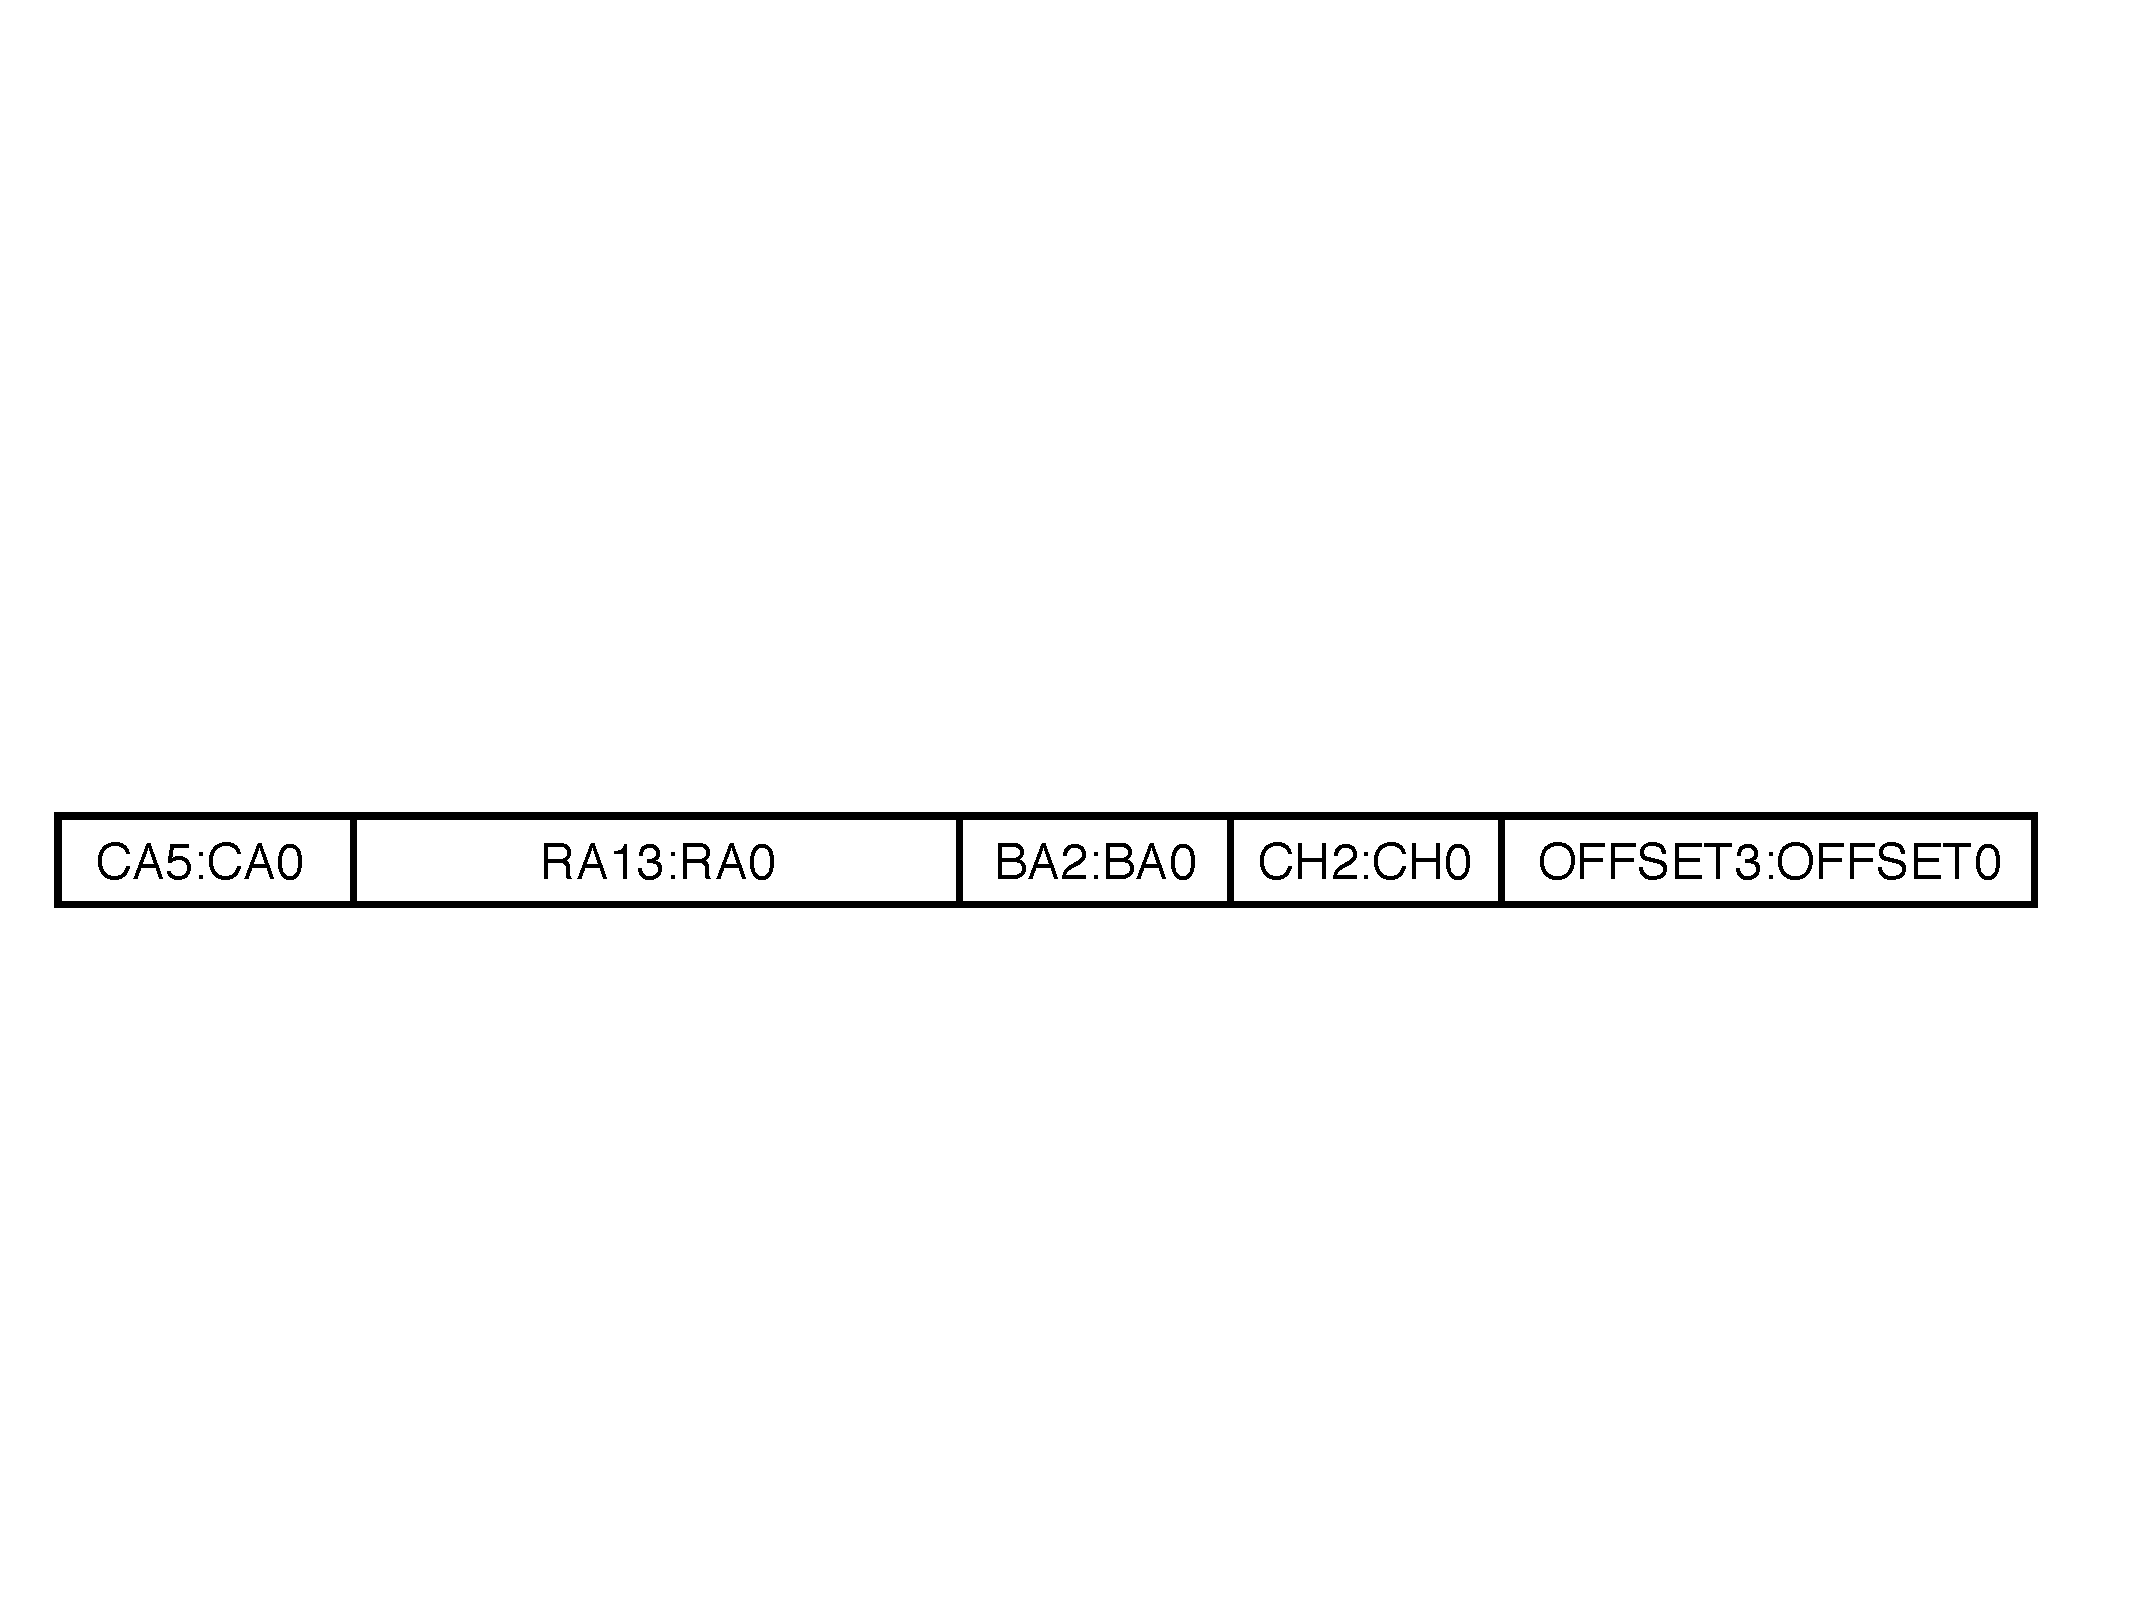
\includegraphics[width=0.98\linewidth]{figures/ChAddressing.pdf} 
\caption{Address mapping for channels.}
\label{fig:mapping}
\end{figure}
%%%%%%%%%%%%%%%%%%%%%%%%%%%%%%%%%%%%%%%%%%%


\begin{figure}[h!] \centering
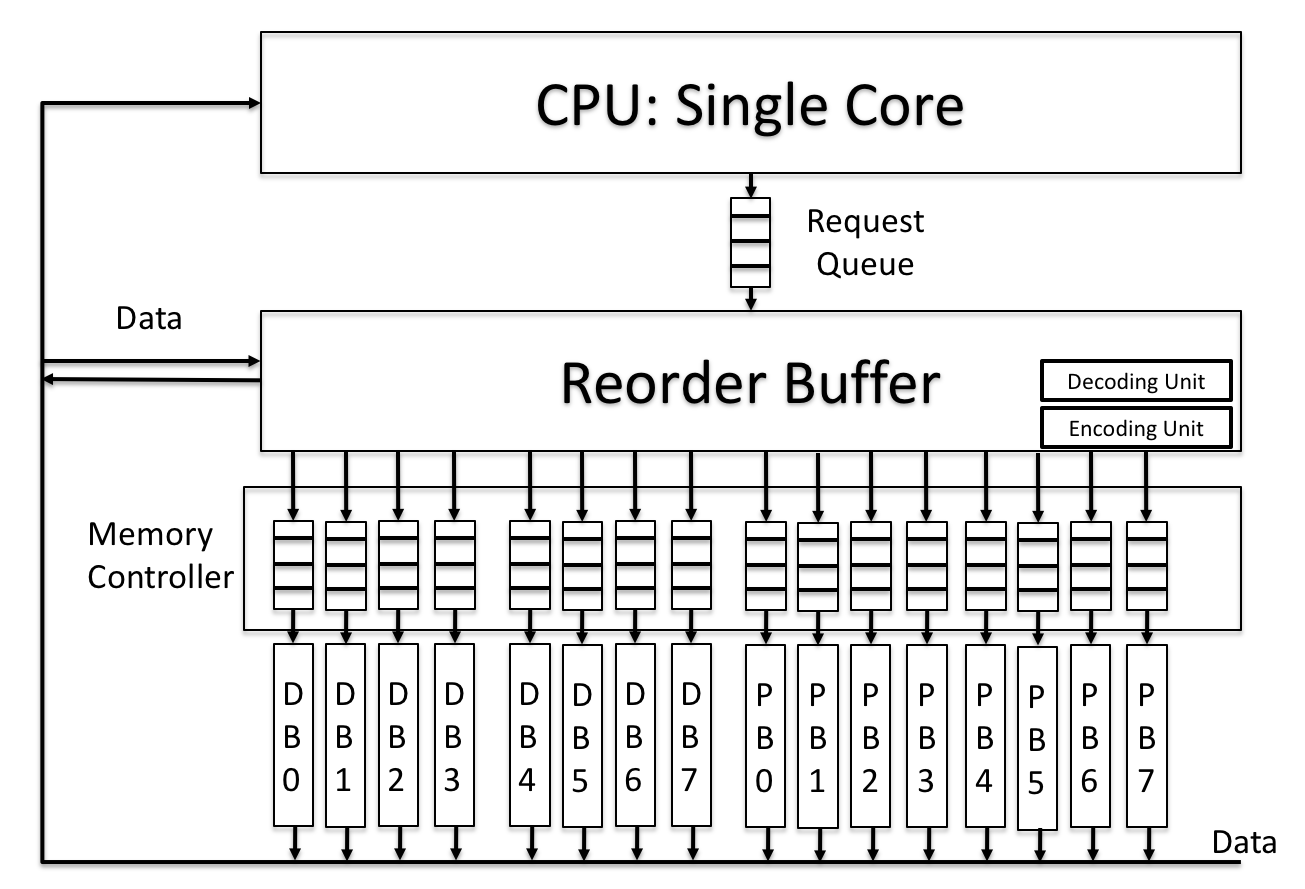
\includegraphics[width=0.9\linewidth]{figures/single-core-cpu.png} 
\caption{Single-core CPU Simulation.}
\label{fig:single-core-cpu}
\end{figure}

\begin{figure}[h!] \centering
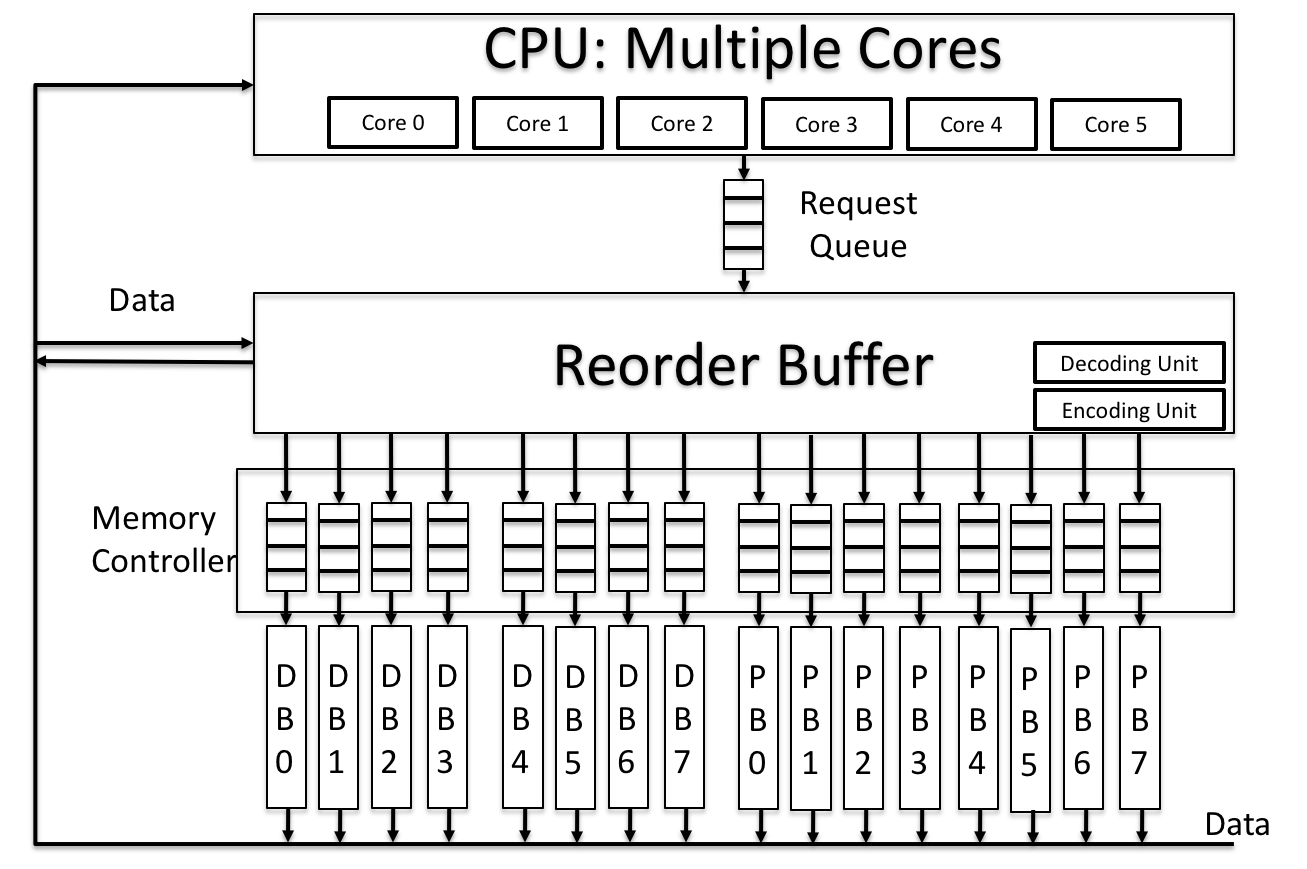
\includegraphics[width=0.9\linewidth]{figures/multi-core-cpu.png} 
\caption{Multi-core CPU Simulation.}
\label{fig:multi-core-cpu}
\end{figure}

\subsection{Memory Traces}
We use the PARSEC benchmark suite to evaluate how the proposed memory system improves performance in shared memory scenarios. The PARSEC benchmark suite was developed to evaluate chip multiprocessors. We run the PARSEC benchmarks on the gem5 simulator to generate memory traces for use in evaluating the efficacy of the proposed memory system. The memory traces we use to evaluate the proposed memory system are dense, as illustrated by Figure~\ref{fig:canneal_dense}. It is necessary that the memory traces we use are dense, otherwise the benefits of the proposed memory system will not be visible.
 
We observe that the regions of memory most heavily used in the trace pictured in Figure~\ref{fig:canneal_dense} are stationary with respect to time. Figure~\ref{fig:canneal_whole} shows an entire memory trace. We observe that there are two major memory bands. Figure~\ref{fig:canneal_dense} is a magnified view of the bottom band. This figure reveals that the bottom band is composed of two sub-bands of similar density. These two sub-bands contain over 90\% of the memory accesses in this memory trace. Figure~\ref{fig:canneal_dense} also shows that the memory regions used by the processors overlap to a degree which yields frequent bank conflicts.

Because the structure of the PARSEC benchmark traces is similar across the benchmarks, we choose to augment the traces in order to analyze how the proposed memory system behaves in more memory access scenarios. We augment the trace by splitting the traces into a greater number of bands, and we introduce a linear ramp. The augmentations we implement are visualized in Figure~\ref{fig:vips_split} and Figure~\ref{fig:vips_ramp}

\begin{figure}[h!]
		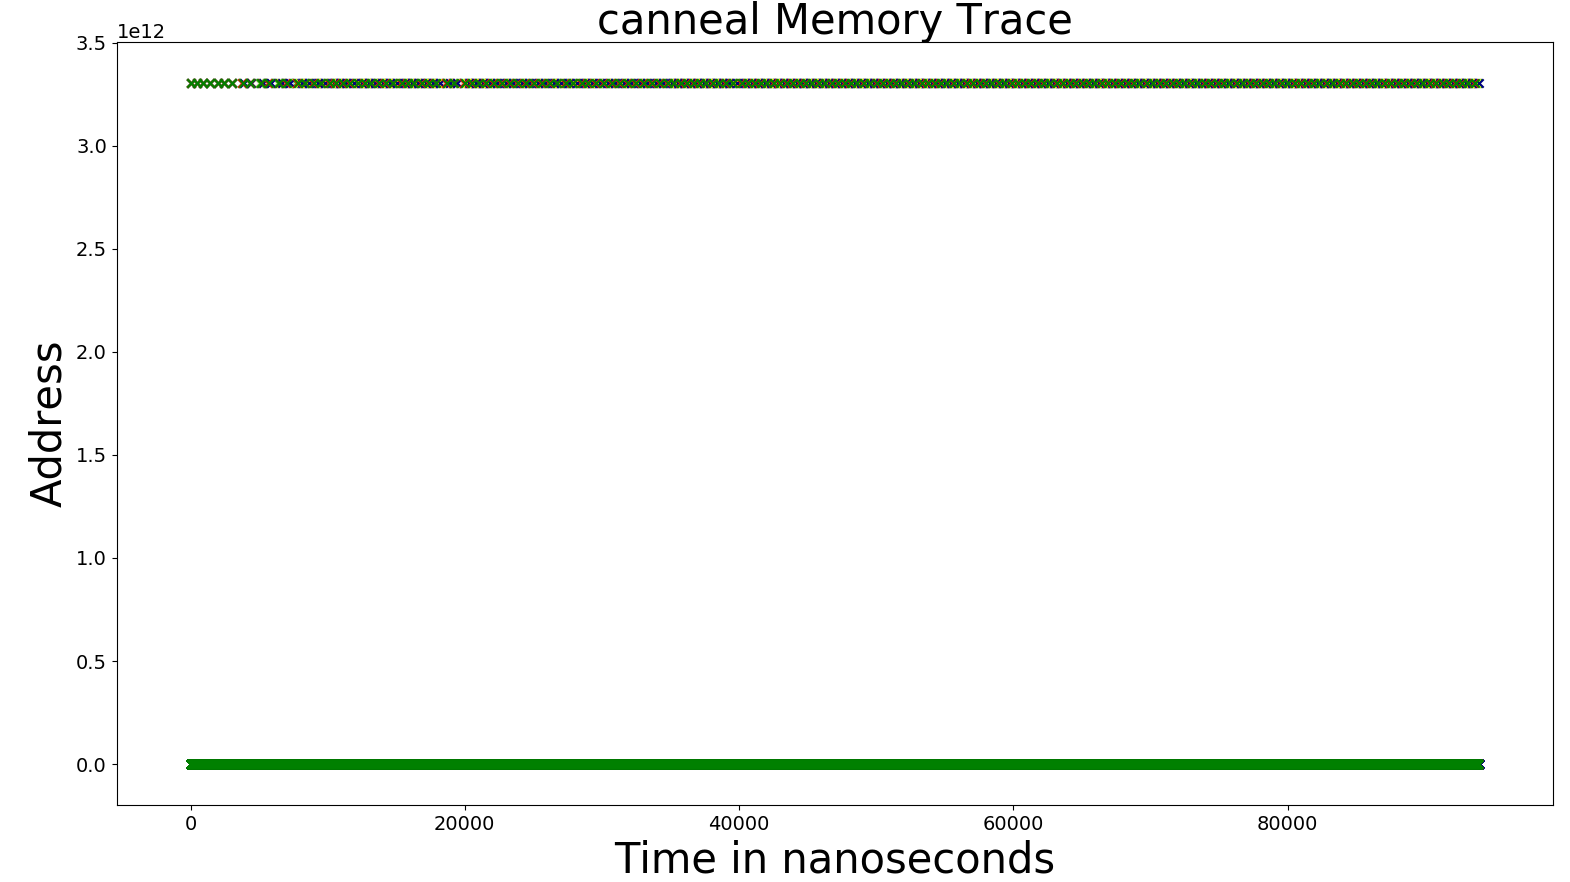
\includegraphics[width=\linewidth]{figures/canneal_whole.png}
		\caption{The entire memory trace of the canneal PARSEC benchmark simulated in gem5.}
		\label{fig:canneal_whole}
\end{figure}

\begin{figure}[h!]
		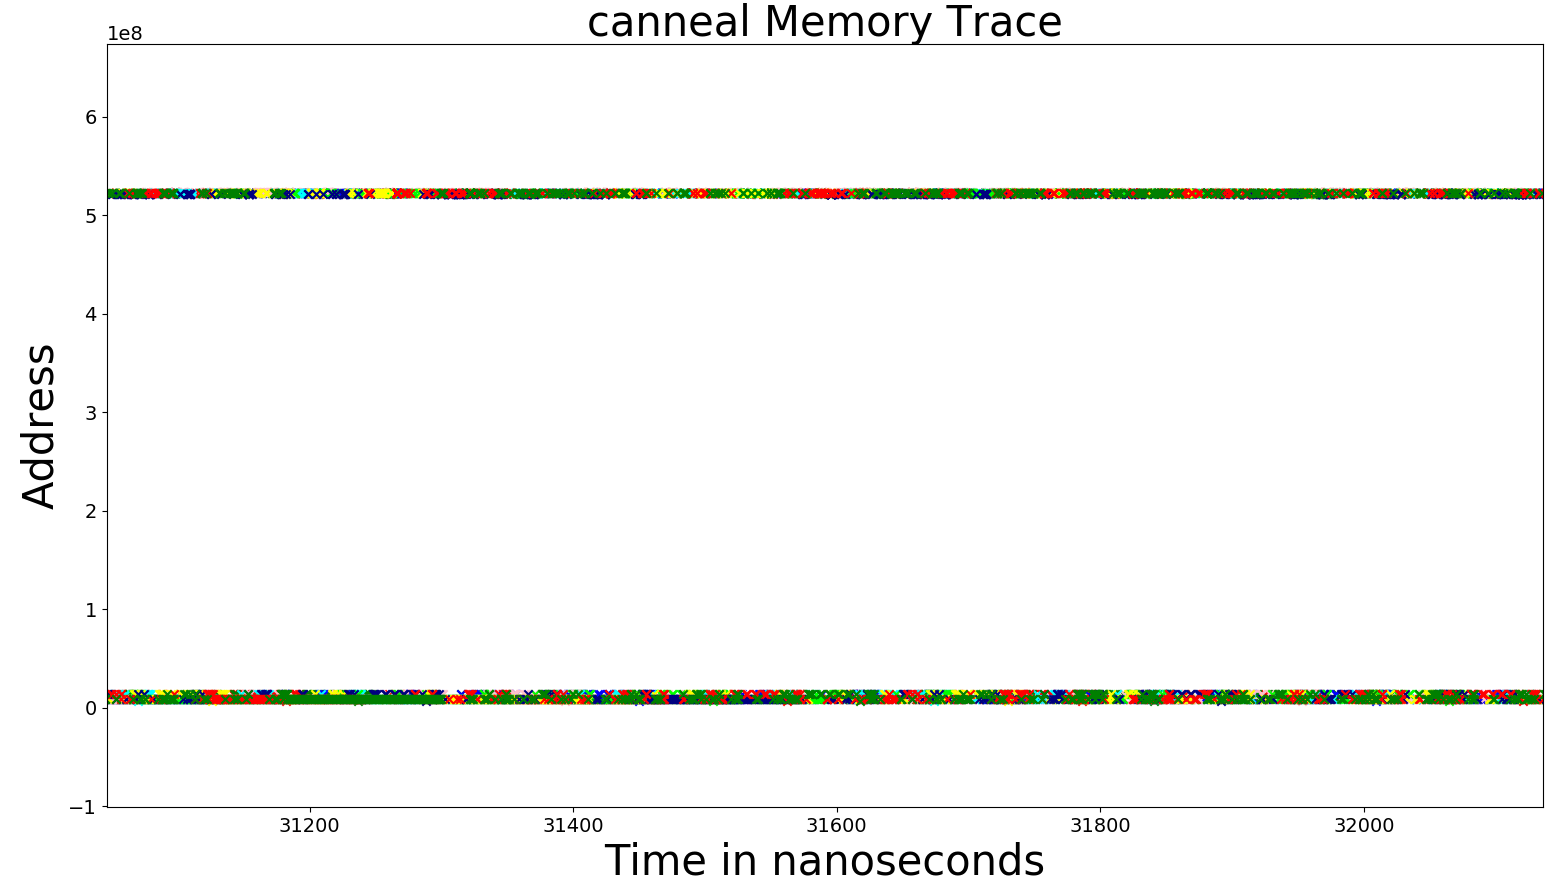
\includegraphics[width=\linewidth]{figures/canneal_trace.png}
		\caption{The bottom band of the trace pictured in Figure~\ref{fig:canneal_whole}. Two sub-bands are visible.}
		\label{fig:canneal_dense}
\end{figure}
		
\begin{figure}[h!]
		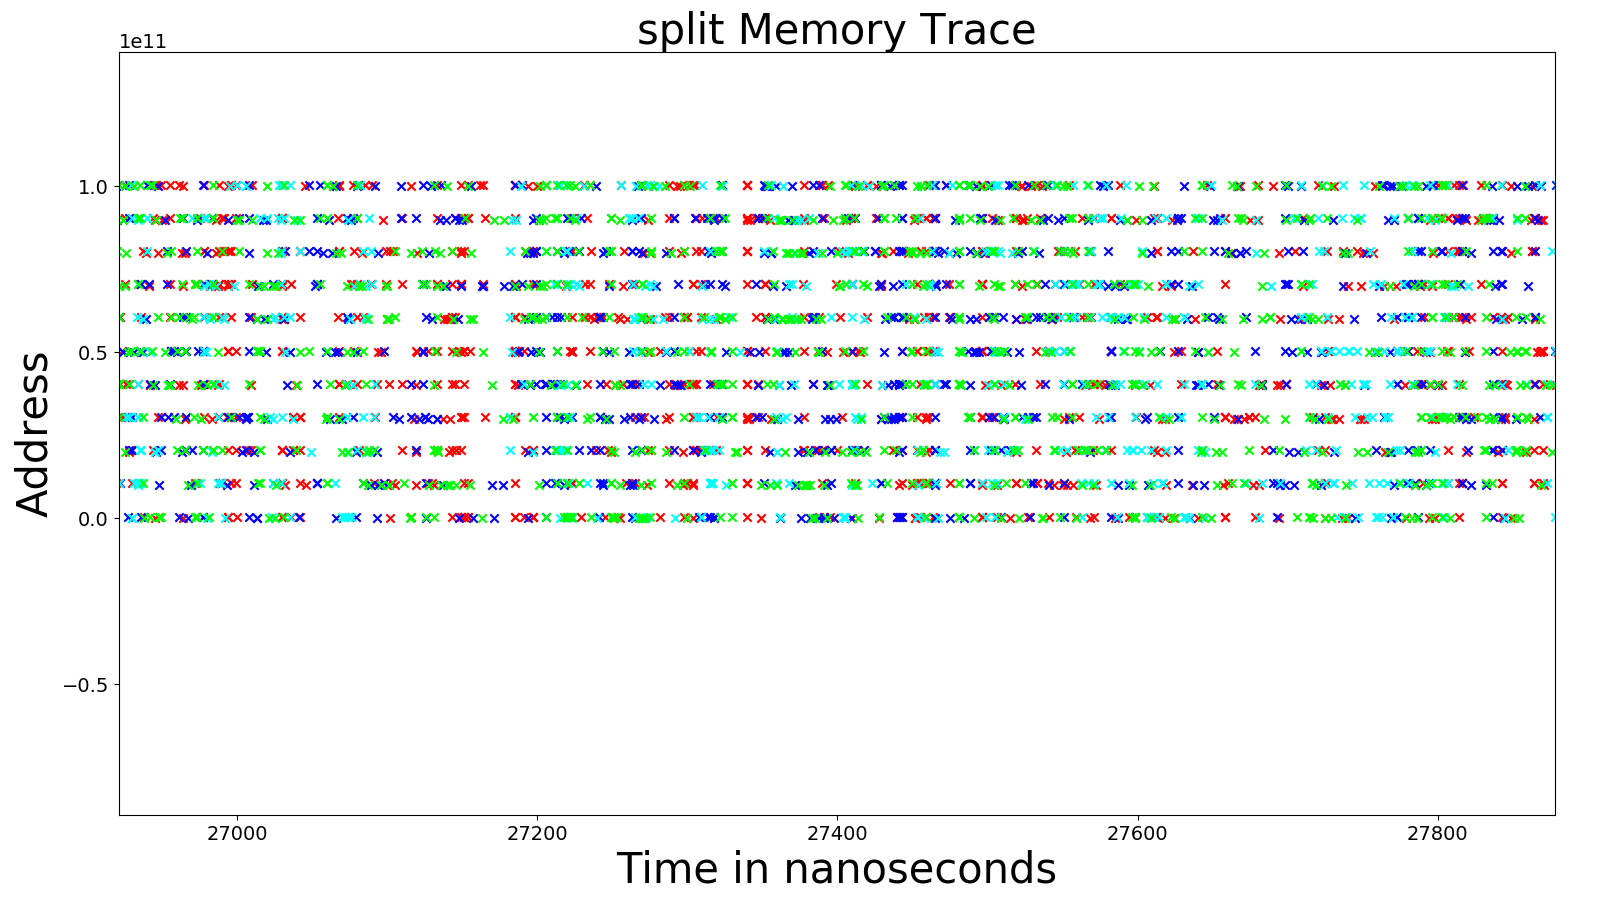
\includegraphics[width=\linewidth]{figures/vips_split.png}
		\caption{A trace of a PARSEC benchmark augmented to increase the number of memory bands.}
		\label{fig:vips_split}
\end{figure}

\begin{figure}[h!]
		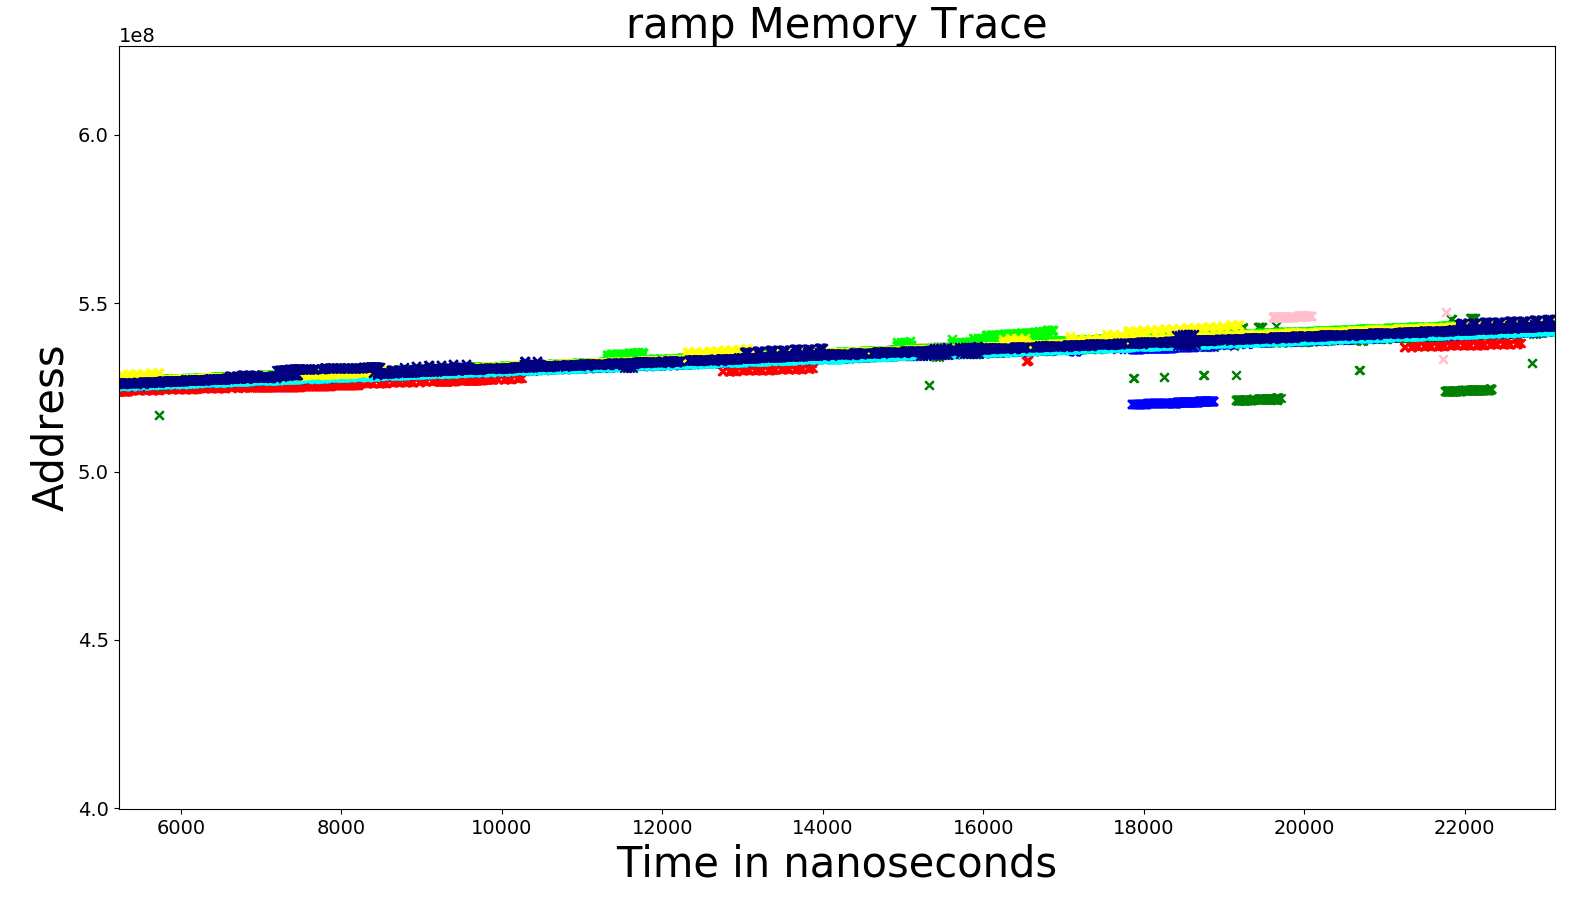
\includegraphics[width=\linewidth]{figures/vips_ramp.png}
		\caption{An PARSEC benchmark trace augmented to include a linear ramp.}
		\label{fig:vips_ramp}
\end{figure}

\subsection{Ramulator Simulations}
The Ramulator program simulates DRAM systems taking a memory trace as input. At the conclusion of a simulation, the number of CPU cycles needed to execute the memory trace is output. We compare the number of CPU cycles required to execute memory traces as simulated by an unmodified version of Ramulator and a version which includes the proposed memory system.

In addition to the 8-bank parity scheme described in Section~\ref{sec:codingArchitecture}, We also examine the efficacy of alternate parity bank schemes. In particular, we employ the following schemes.
\begin{itemize}
	\item 8-banks 4-message symbols: The scheme described in Section~\ref{sec:codingArchitecture}.
	\item 4-banks 4-message symbols: A scheme which consists of the first four banks of the scheme described in Section~\ref{sec:codingArchitecture}.
	\item 8-bank duplicate: A scheme which consists of duplicates of the original eight data banks. The parity banks in this scheme are not parity banks per se, as they do not contain parity elements.
	\item 12-bank 2-message symbols: A scheme constructed by partitioning the data banks into two groups of four banks, and generating 6 parity banks from each combination of two banks from each of the disjoint groups.
\end{itemize}

\subsection{Simulation Results}
\label{sec:results}
The proposed memory system performs consistently well across the PARSEC 2.1v and 3.0v benchmarks. We find that the parity structure has a small impact on the performance of the system, and the reorder buffer length is  the critical factor for determining the efficacy of a system. In several scenarios we show greater than 50\% reduction of CPU cycles needed for the simulation to complete. In the figure below, we show the number of simulated CPU cycles for the proposed memory system compared to the number of simulated CPU cycles for the baseline coded system. A speedup coefficient is calculated by dividing the simulated CPU cycle count by the baseline CPU cycle count. Most notable in these results is that a short reorder buffer length of 8 is sufficient to achieve significant improvement, and once the reorder buffer reaches a certain length the marginal benefits of increasing buffer length diminish.

\begin{figure}[h!]
		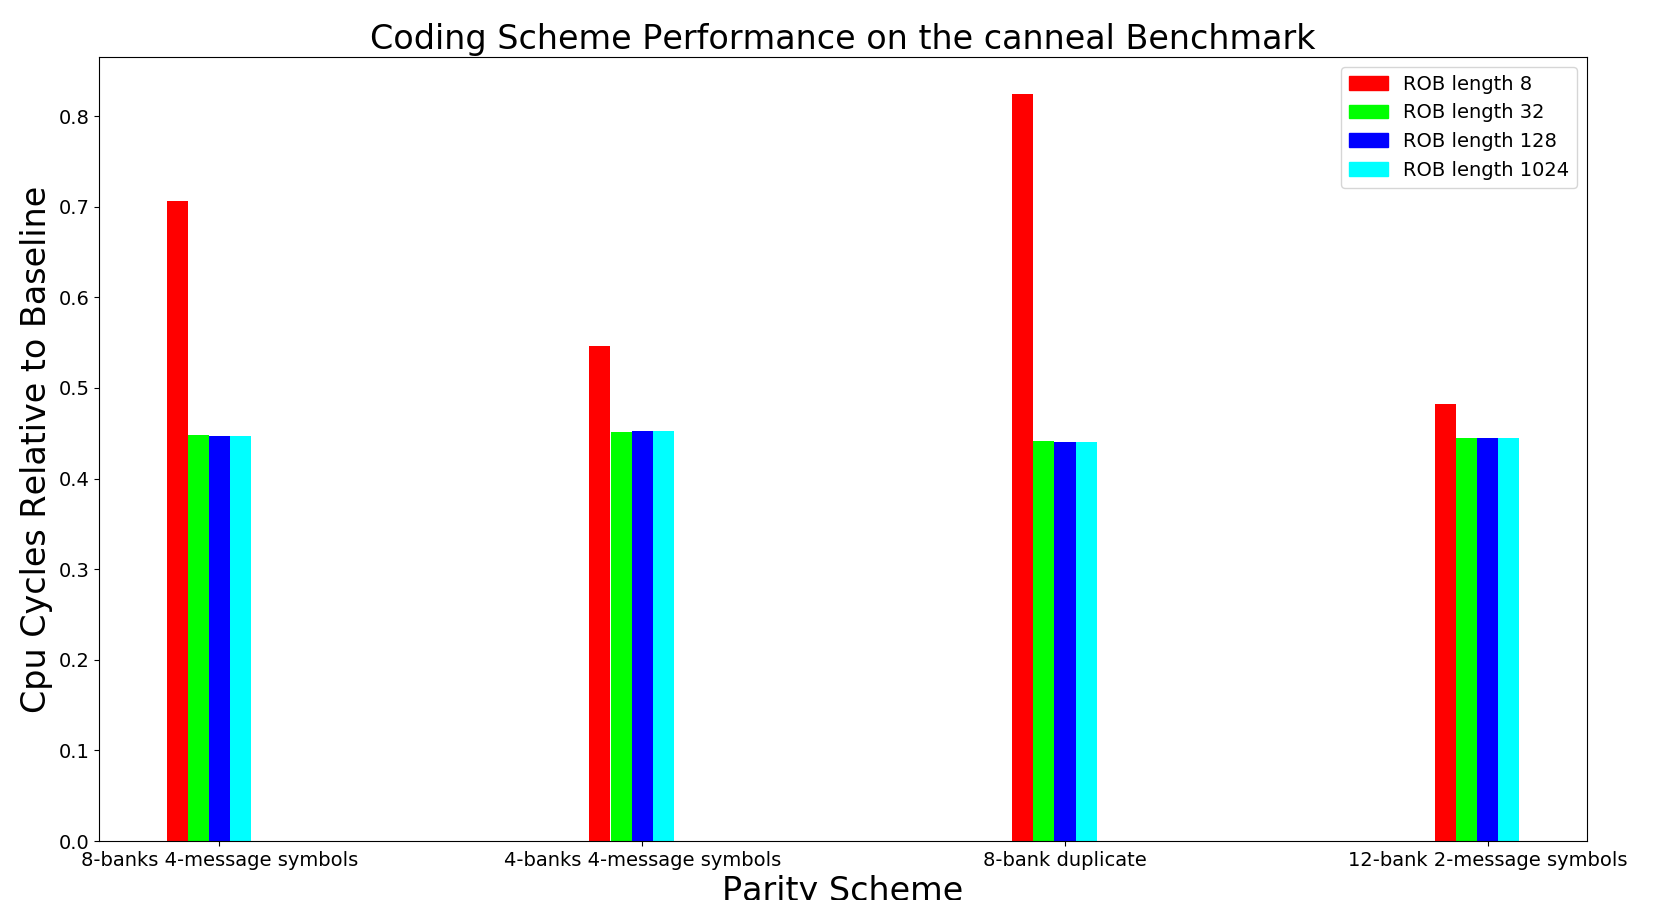
\includegraphics[width=\linewidth]{figures/canneal_results.png}
		\caption{The performance of the proposed coded system on the trace pictured in Figure~\ref{fig:canneal_results}.}
		\label{fig:canneal_results}
\end{figure}
		

\subsection{Augmented PARSEC Results}
\label{sec:aug_results}

The augmentations on the PARSEC traces significantly impact how the proposed memory system performs. Figure~\ref{fig:vips_split_results} shows the simulation results for the benchmark pictured in Figure~\ref{fig:vips_split}. The results show that the proposed coded system is able to achieve improvements similar to those picture in Figure~\ref{fig:canneal_results}, however a larger reorder buffer length is needed to achieve these results. Figure~\ref{fig:vips_ramp_results} shows that memory traces with linear ramps benefit less from the proposed memory system. We again see that a larger reorder buffer length is needed to maximize the performance of the system, but the overall performance improvement is less than those pictured in Figure~\ref{fig:canneal_results}. The parity scheme has a greater impact on performance for the augmented PARSEC traces, as the results show that the exclusion of parity banks leads to worse performance. 

\begin{figure}[h!]
		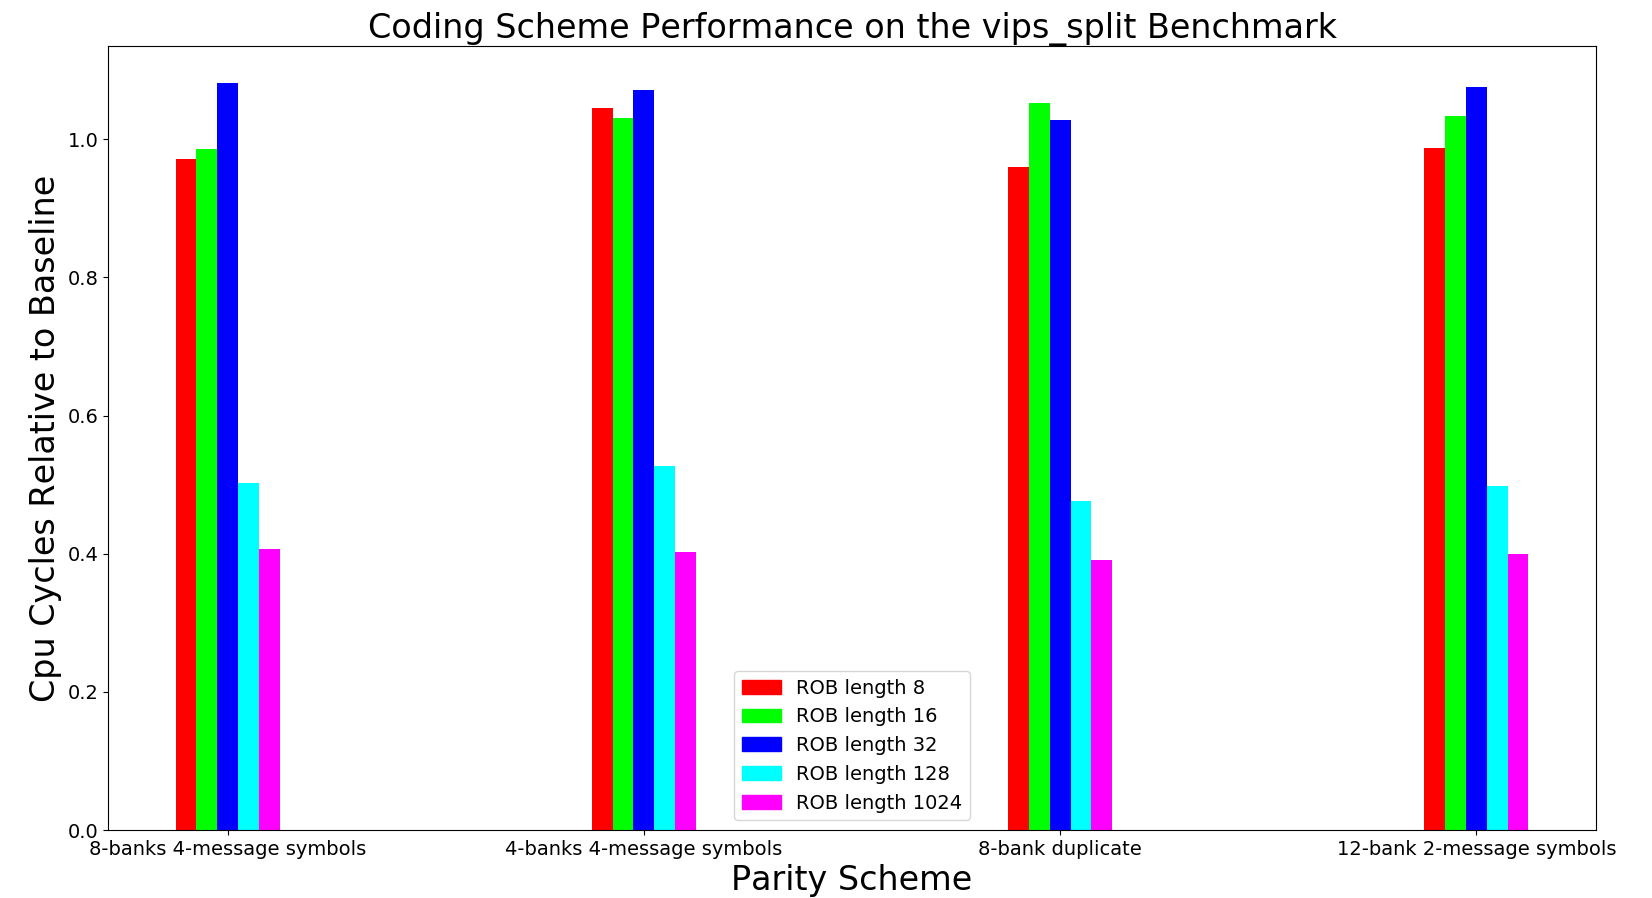
\includegraphics[width=\linewidth]{figures/vips_split_results.png}
		\caption{The performance of the proposed coded system on the trace pictured in Figure~\ref{fig:vips_split}.}
		\label{fig:vips_split_results}
\end{figure}


\begin{figure}[h!]
		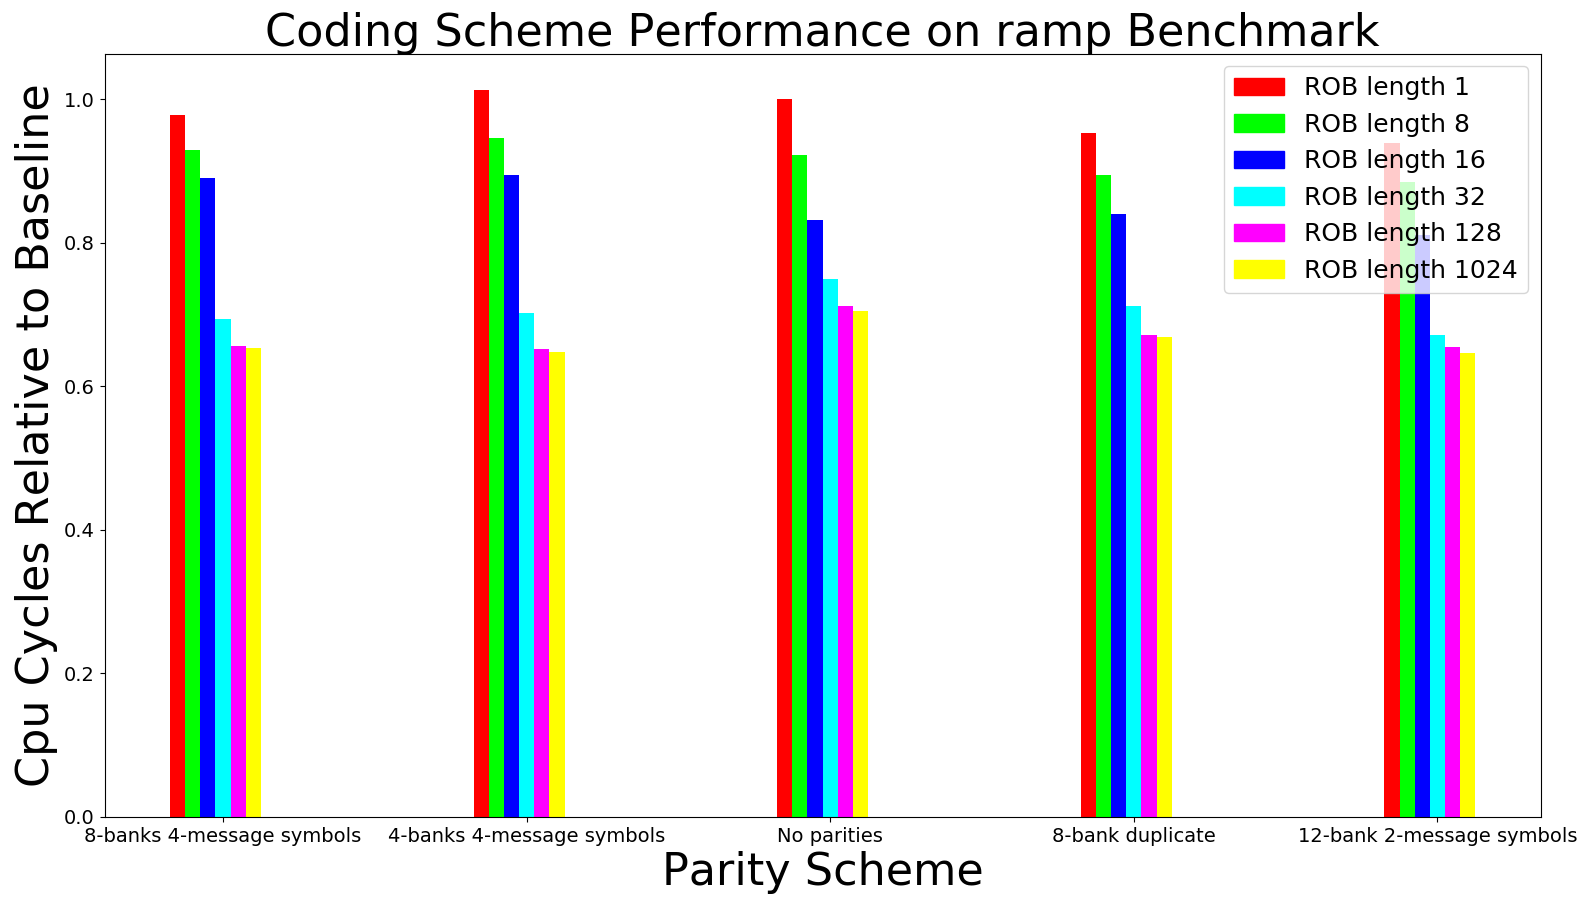
\includegraphics[width=\linewidth]{figures/vips_ramp_results.png}
		\caption{The performance of the proposed coded system on the trace pictured in Figure~\ref{fig:vips_ramp}.}
		\label{fig:vips_ramp_results}
\end{figure}